
\documentclass[11pt]{article}
 
\usepackage[margin=1in]{geometry} 
\usepackage{amsmath,amsthm,amssymb,scrextend}
\usepackage{fancyhdr}
\pagestyle{fancy}

\newcommand{\cont}{\subseteq}
\usepackage{csvsimple}
\usepackage{tikz}
\usepackage{pgfplots}
\usepackage{amsmath}
\usepackage[mathscr]{euscript}
\let\euscr\mathscr \let\mathscr\relax% just so we can load this and rsfs
\usepackage[scr]{rsfso}
\usepackage{amsthm}
\usepackage{amssymb}
\usepackage{multicol}
\usepackage[colorlinks=true, pdfstartview=FitV, linkcolor=blue,
citecolor=blue, urlcolor=blue]{hyperref}

\usepackage{setspace}
\onehalfspacing

\usepackage{siunitx} % 用于处理数字和单位


\DeclareMathOperator{\arcsec}{arcsec}
\DeclareMathOperator{\arccot}{arccot}
\DeclareMathOperator{\arccsc}{arccsc}
\newcommand{\ddx}{\frac{d}{dx}}
\newcommand{\dfdx}{\frac{df}{dx}}
\newcommand{\ddxp}[1]{\frac{d}{dx}\left( #1 \right)}
\newcommand{\dydx}{\frac{dy}{dx}}
\let\ds\displaystyle
\newcommand{\intx}[1]{\int #1 \, dx}
\newcommand{\intt}[1]{\int #1 \, dt}
\newcommand{\defint}[3]{\int_{#1}^{#2} #3 \, dx}
\newcommand{\imp}{\Rightarrow}
\newcommand{\un}{\cup}
\newcommand{\inter}{\cap}
\newcommand{\ps}{\mathscr{P}}
\newcommand{\set}[1]{\left\{ #1 \right\}}
\newtheorem*{sol}{Solution}
\newtheorem*{claim}{Claim}

\newcounter{question}
\newenvironment{Question}{%
    \stepcounter{question}%
    \textbf{Question (\alph{question})}%
}{}

\usepackage[most]{tcolorbox} % 引入 tcolorbox 宏包
\newtcolorbox{claimbox}{
  colback=blue!5!white, % 背景颜色
  colframe=blue!50!black, % 边框颜色
  title=Claim, % 框标题
  fonttitle=\bfseries, % 标题字体加粗
  arc=1mm, % 边角弧度
  outer arc=1mm, % 外边角弧度
  top=2mm, % 顶部内边距
  bottom=2mm % 底部内边距
}

\newtcolorbox{warningbox}{
  colback=yellow!5!white, % 背景颜色
  colframe=yellow!55!gray, % 边框颜色
  title=Warning, % 框标题
  fonttitle=\bfseries, % 标题字体加粗
  arc=1mm, % 边角弧度
  outer arc=1mm, % 外边角弧度
  top=2mm, % 顶部内边距
  bottom=2mm % 底部内边距
}



\begin{document}
 
% EVERYTHING ABOVE THIS LINE IS JUST PREABLE, NO NEED TO MESS WITH IT.__________________________________________________________________________________________
%

\lhead{FIN3080 Assignment 4}
\chead{LIU, Junle \ 122090337}
\rhead{\today}

% \maketitle
\begin{spacing}{1.5}


\section*{Problem 1}

\noindent
\textbf{Overview}

The overall steps are given in the homework instruction. In this report I will discuss about some detailed manipulations and show the study results.

\noindent
\textbf{Data Collection}

The data are all downloaded from CSMAR as required by the problem, namely the Daily Market Returns, Daily Stock Price Returns, Index per Share, Statements Release Dates over 2016 to 2022 (some data in 2014 and 2015 are included for window operations).



\noindent
\textbf{Step 1 \& 2} 

The data is downloaded and read as DataFrame as required. Noted that there are so many files if we choose .csv files. `.concat' function can easily combine these files together in y axis. The columns are renamed accordingly as well.


\noindent
\textbf{Step 3} 

The EPS file is read and converted to DataFrame. Because excluding parent statements is required, all the rows with `statement\_type' are deleted.

\begin{claimbox}
  On step 3.3, the instruction requires to delete stock names starting with ST and PT. However, some stocks names may coincidentally start with PT/ST (e.g. 836871.BJ PTE). Therefore, I use the Chinese version of stock names, and deleted all stocks starting with ST, PT, *ST, SST, S*ST (once they have such prefix in one period, I delete the company completely).
\end{claimbox}

Then step 3.4 -- 3.6 are some time manipulation procedure, with the usage of pd.to\_datetime \& to\_period. 

\begin{warningbox}
  On step 3.7 \& 3.8, we can NOT directly use `.shift()', because there exists cases that the downloaded data only include December EPS at some random years. So the data can be completely messy if using `.groupby()' + `.shift()' or `.diff()'.
\end{warningbox}

Thus, step 3.7 \& 3.8 are rather complex. I first extract EPS values for June and December in the same year, then calculates the difference between December EPS and June EPS, reflecting the EPS change for the second half of the fiscal year. This result replaces the original December EPS in the data. Noted that the code processes this calculation by grouping the data by stock code and applying these functions to each group, updating the entire dataset accordingly.

Continue on step 3.9, now `.shift()' can be used, because step 3.8 ensures that the data is well structured (all the years with only one entry data will be discarded because of `.dropna()')

Steps3.11 -- 3.13 are steps for correctly derive the SUE deciles. Noted that `.pivot()' is used for converting the long DataFrame to wide DataFrame.

\begin{claimbox}
  On Step 3.9, UE's from the subtraction of this year’s EPS with last year’s. As 2014h1 \& 2014h2 do not have ``last year” in the data set, so their UE will be NaN. On Step 3.10, we include the recent three periods’ data as the window for s.d. Thus, 2015h1, 2015h2 and 2016h1 will be used to get s.d. for 2016h2, and these three periods will not have their own SUE, instead they are NaN and be discarded. That's why the wide data set of EPS from Step 3.13 may start with 2016h2 instead of 2016h1.
\end{claimbox}


\noindent
\textbf{Step 4} 

Very similar to the process to get wide DataFrame in step 3.13, with an additional step to convert the body data into datetime. 


\noindent
\textbf{Step 5} 

All the useful DataFrame we got above are combined into a wide one using `pd.merge()'.


\noindent
\textbf{Step 6} 

Step 6.3 is complex. It uses a loop for iterating on every time period column. The implementation follows the method 2 to get event day in the tutorial slide. For each iteration, the NaN data will be discarded, then the cumulative return of each decile is calculated using `.cumsum()'.

\begin{warningbox}
  Directly using the method on tutorial may cause some time disruption due to unexpected trading suspension (without PT/ST labeled, e.g 000716.SZ). Thus, I limited the original trading date range before getting the relative trading date difference. Data out of range will be discarded for data accuracy.
\end{warningbox}

On step 6.4, we get the mean of decile cumulative return of all half-year periods, namely `mean\_portfolio\_car'. Finally we can get the result figure of this event study:


\begin{figure}[ht]
\centering
% \vspace{-0.43cm}
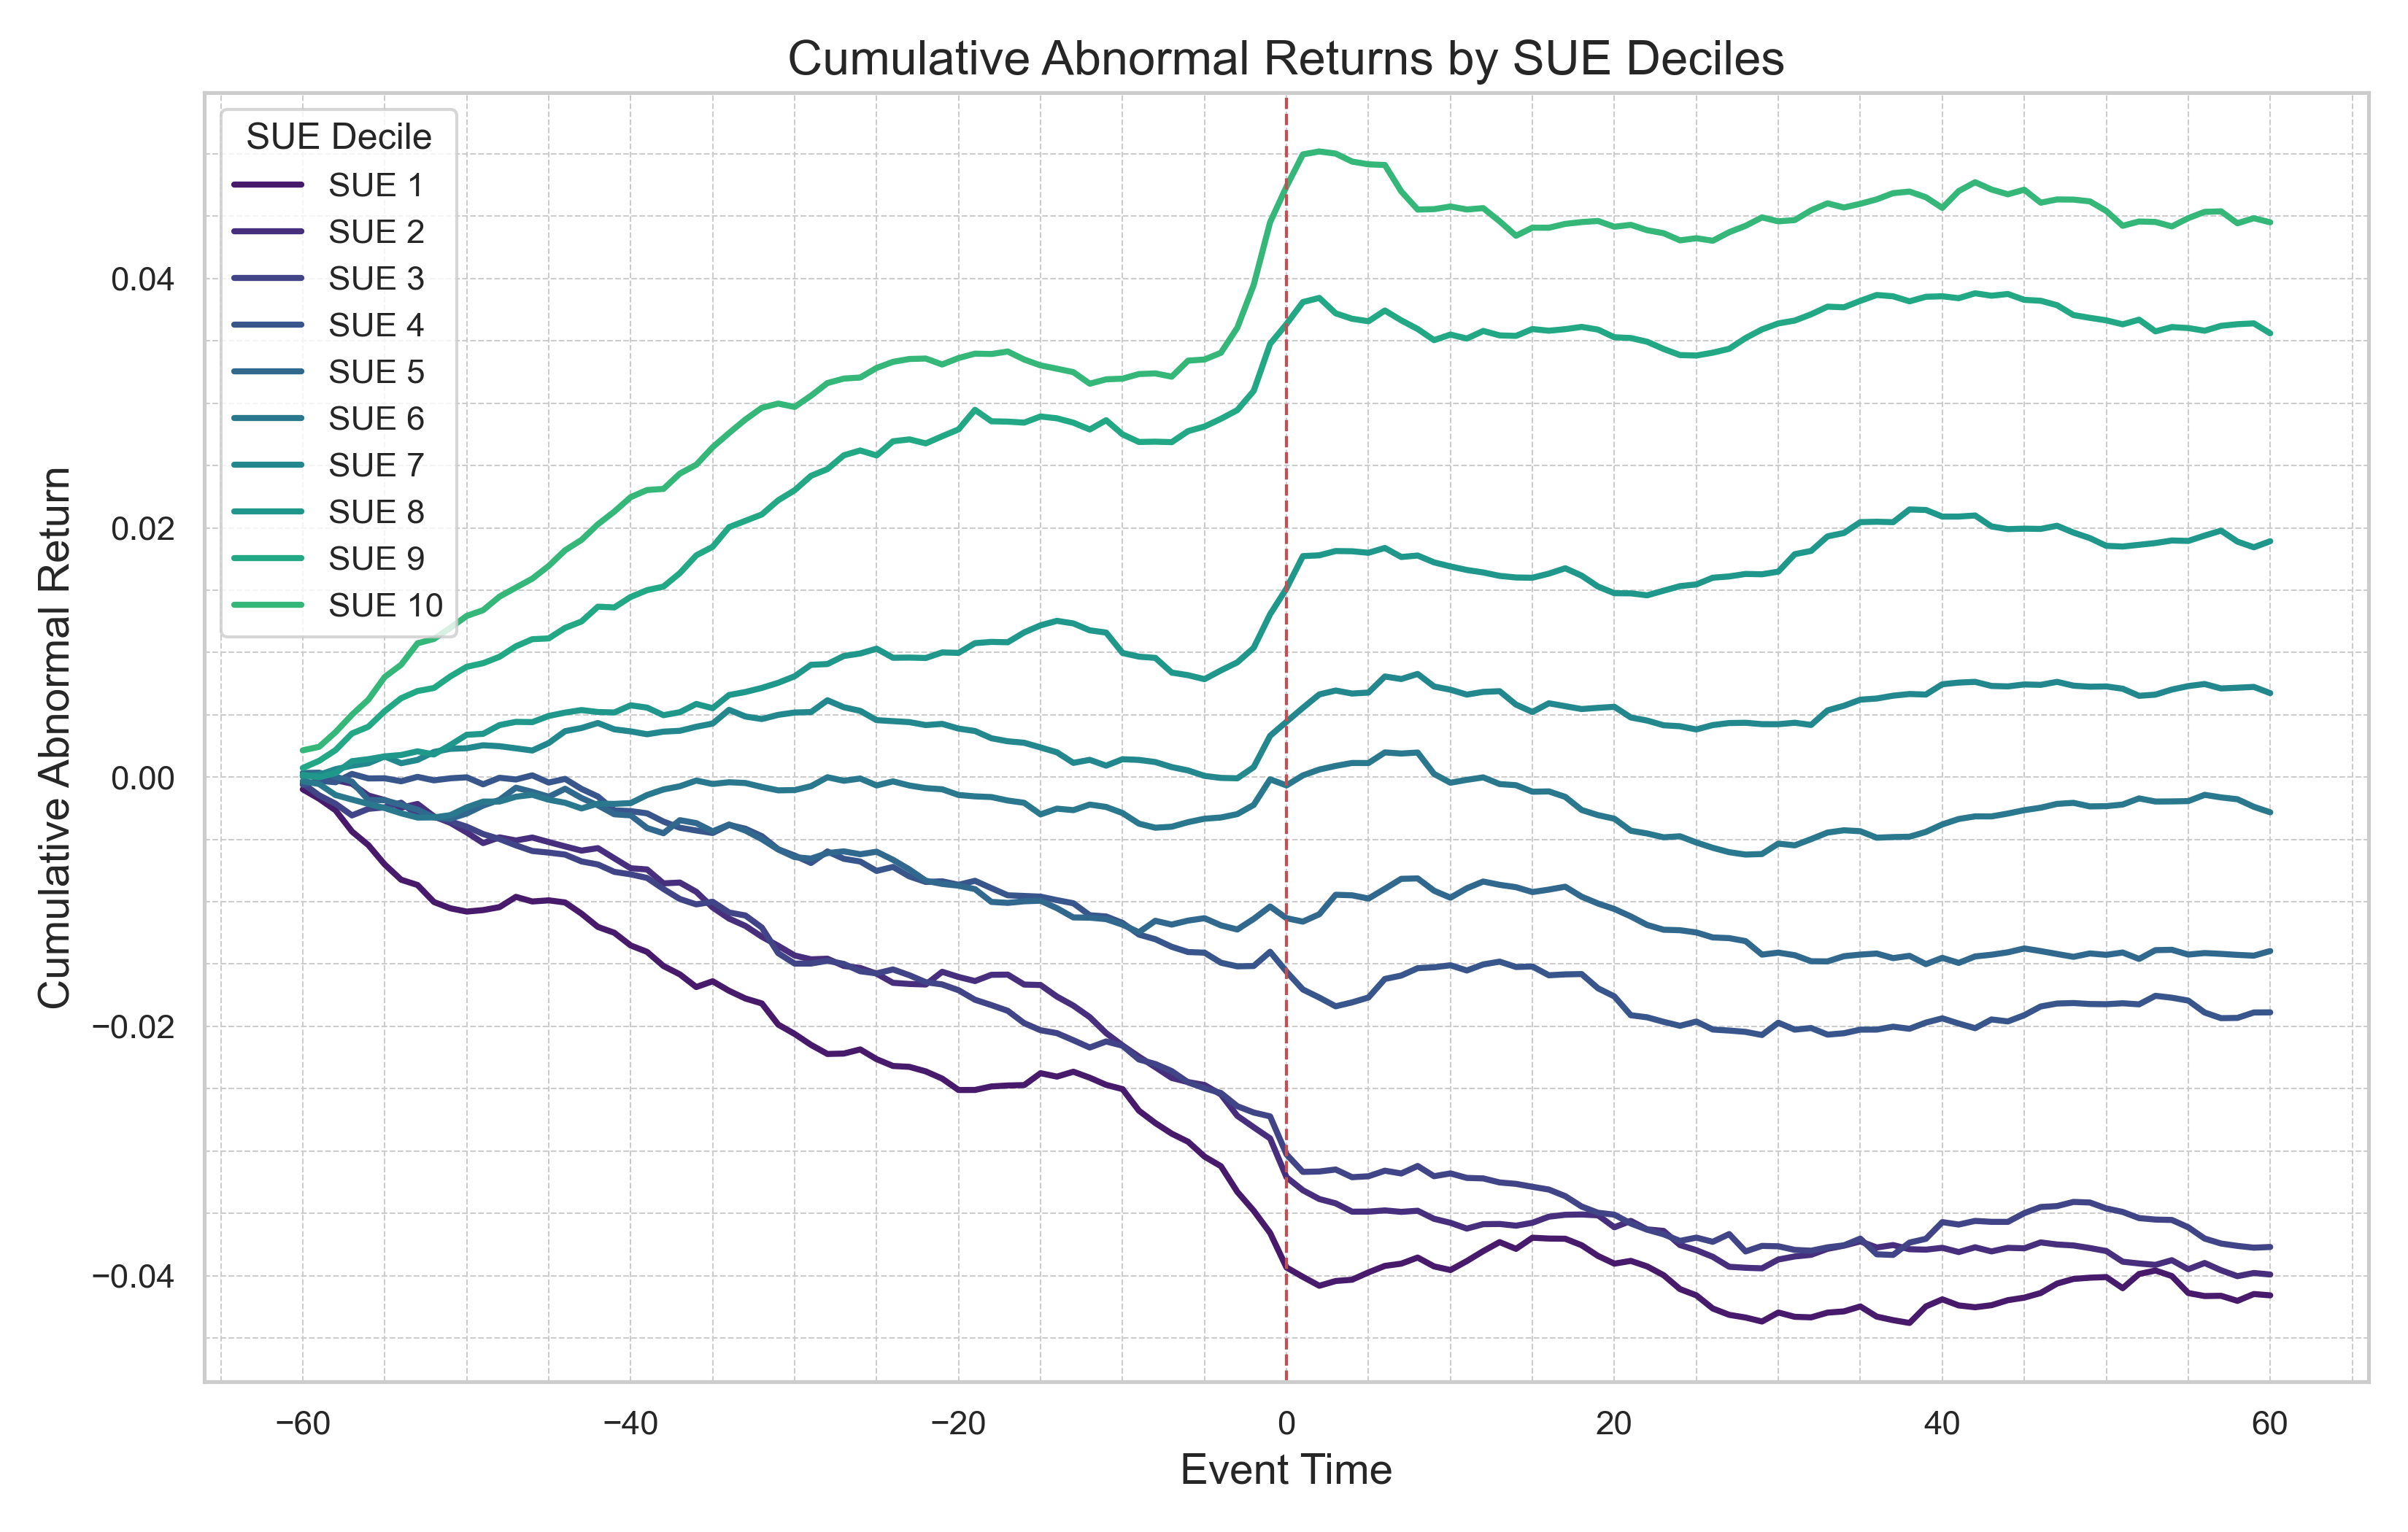
\includegraphics[width=1\textwidth]{data/Result Figure.png}
\caption{Cumulative Abnormal Returns by SUE Deciles}
\label{fig:example}
\end{figure}


\noindent
\textbf{Results}

As shown in the figure, the diciles with higher SUE (SUE 6 -- 10) has higher cumulative abnormal returns with increasing trends; the diciles with lower SUE (SUE 1 -- 4) has lower (more negative) cumulative abnormal returns with decreasing trends.

In conclusion, Post Earnings Announcement Drift (PEAD) exists in China’s A-share markets.


\vspace{1.5cm}

\centering -- END --

\end{spacing}

 


% THE DOCUMENT IS ESSENTIALLY DONE AT THIS POINT, NO NEED TO EDIT ANYTHING BELOW THIS______________________________________________________________________________________________

\end{document}